\underline{Fraktale} są to obiekty geometryczne, których wzorce powtarzają się w różnych skalach. Mimo nietrywialnej struktury w każdej skali mają względnie prostą definicję rekurencyjną.

Gdy sygnały o nieregularnym charakterze (ruchy Browna, kształty w geologii, szeregi czasowe w medycynie) i ich wykresy są zbiorami fraktalnymi w $ R^2 $ - określa się te sygnały jako funkcje fraktalne.

Funkcje takie są samoafiniczne: są samopodobne gdy się je przekształca za pomocą anizotropowego skalowania:

$ f(x) $ jest funkcją samoafiniczną gdy $\forall x_0 \in {\rm I\!R},\space \exists H \in {\rm I\!R}, \lambda > 0 $ takie, że:\newline
$ f(x_0 + \lambda x) - f(x_0) \approx \lambda^H \big[ f(x_0+x) - f(x_0)\big] $, gdzie:\newline
$ H $ - wykładnik Hursta będący miarą chropowatości funkcji. Wykres funkcji jest samopodobny jeśli $ H = 1 $.

Funkcję fraktalne są zazwyczaj \underline{multifraktalne} - ich własności zmieniają się od punktu do punktu: \newline
$ |f(x+l) - f(x)| \propto l^{h(x)}$, gdzie:\newline
$ h(x) $ - wykładnik Holdera funkcji $ f $ punkcie $ x $.

Multifraktalność polega na tym, że dla każdej wartości argumentu $ x $ funkcji $ f(x) $ możemy mieć inny wykładnik Holdera.

\underline{Wymiar fraktalny} $ d $ jest definiowany jako:\newline
$ N = M^d $,\newline
$ d = \dfrac{\ln N}{\ln M} $, gdzie:\newline
$ N $ - ilość powstałych części podczas kroku konstrukcyjnego,\newline
$ M $ - ułamek liniowej długości nowej części w procesie konstrukcji do liniowej długości części pierwotnej.

Np. dla zbioru Cantora $ N = 2 $, $ M = 3 $, $ d = \dfrac{\ln 2}{\ln 3} \approx 0.63 $ (rys.~\ref{cantor}).
\begin{figure} [H]
	\centering
	\begin{subfigure}{.99\textwidth}
		\centering
		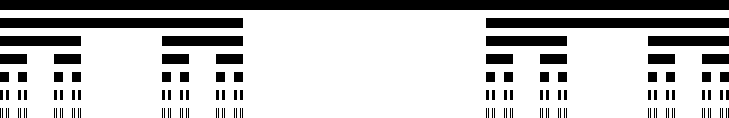
\includegraphics[width=1.0\linewidth]{EDMIIssues/Figures/cantor.png}
	\end{subfigure}
	\caption{Kolejne kroki konstrukcyjne zbioru Cantora.}
	\label{cantor}
\end{figure}

\underline{Multifraktalna analiza szeregów muzycznych}

Melodia i rytm są dwoma podstawowymi cechami utworu muzycznego. Melodia jest sekwencją zmian wysokości dźwięku. Rytm jest sekwencją długości trwania dźwięków melodii. Melodię odwzorowuje się na rozkład punktów, dzieląc oktawę równomiernie na 12 wysokości tonu.

Konwersja zapisu muzycznego na szeregi punktowe (przykład na rysunku~\ref{gavotte}):
\begin{itemize}
	\item pierwszy dźwięk melodii przyjmuje się jako podstawowy i stawia sie punkt na pierwszej pozycji, na osi poziomej
	\item jeśli różnica wysokości dźwięku drugiego wynosi $ m $ stawia się punkt na pozycji $ 1 + m $
\end{itemize}

Podobnie postępujemy z rytmem. Wybieramy najniższą miarę czasu (np. szesnastka). Jeśli $ m $ to różnica odległości koleljnego dźwięku od poprzedniego w szeregu miar czasowym, to stawiamy punkt w miejscu oddalonym o $ m $ od poprzedniego Różnica pomiędzy szesnstką a ósemką to 1, szesnastką, a ćwierćnutą - 2 itd.

\begin{figure} [H]
	\centering
	\begin{subfigure}{.8\textwidth}
		\centering
		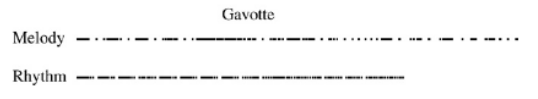
\includegraphics[width=1.0\linewidth]{EDMIIssues/Figures/gavotte.png}
	\end{subfigure}
	\caption{Konwersja utworu \textit{Gavotte} na szeregi punktowe.}
	\label{gavotte}
\end{figure} 

Obliczanie wykładnika Holdera:
\begin{itemize}
	\item wybieramy punkt $ i $ na osi poziomej (zaczerniony bądź pusty)
	\item zliczamy liczbę punktów $ p_i $ w pokryciu o promieniu $ r $ i wyliczamy rozkład $ p_i(r) $, zmieniając wartość $ r $,
	\item wykładnik Holdera dany jest jako nachylenie funkcji $ p_i(r) $ w skali $ \log-\log $,
	\item przsuwając sie po szeregu punktowym, otrzymujemy zależność wykładnika od położenia $ i $.
\end{itemize} 
\textbf{Wnioski}:
\begin{itemize}
	\item Utwory muzyczne posiadają własności multifraktalne.
	\item Metoda pozwala segregować utwory muzyczne ze względu na własności melodi oraz ze względu na rytmikę utworu.
	\item Oba szeregi można połączyć, tworząc unikatową charakterystykę każdego utworu - otrzymuje się fraktal podobny do schodków diabelskich (rys.~\ref{stairs}).
\end{itemize}

\begin{figure} [H]
	\centering
	\begin{subfigure}{.8\textwidth}
		\centering
		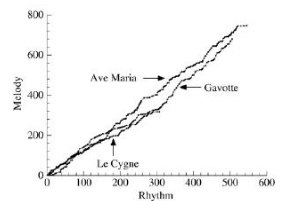
\includegraphics[width=1.0\linewidth]{EDMIIssues/Figures/stairs.png}
	\end{subfigure}
	\caption{Przykłady połączonych konwersji dla rytmu i melodii.}
	\label{stairs}
\end{figure} 

\underline{Multifraktalna analiza beztrendowa (uogólniona multifraktalna procedura DFA)}

\begin{itemize}
	\item Dzielimy sygnał na $ k $ segmentów o długości $ s $,
	\item Dla każdego segmentu wykonuję się regresję (liniową lub nieliniową) i odejmuje się jej wynik od sygnału w segmencie
	\item dla różnych długości segmentu $ s $ oraz różnych wartości parametru $ q $ oblicza się miarę fluktuacji zdefiniowaną następująco:\newline
	$ F_q(s) = \dfrac{1}{2N_s} \bigg[\sum\limits_{v=1}^{2N_s} F^2(v, s)^{\frac{q}{2}} \bigg]^{\frac{1}{q}} $, gdzie:\newline
	$ v $ - indeks okna,\newline
	$ q $ - parametr, jeśli $ q < 0 $ - małe fluktuację, jeśli $ q > 0 $ - duże.
	\item plotuje się wyniki w skali log-log (rys.~\ref{dfa})
	\item jeśli analizowany sygnał jest daleko-zasięgowo skolerowany według prawa potęgowego wtedy $ F_q(s) \propto s^{h(q)} $, gdzie $ h $ - uogólniony wykładnik Hursta.
\end{itemize}

\begin{figure} [H]
	\centering
	\begin{subfigure}{.8\textwidth}
		\centering
		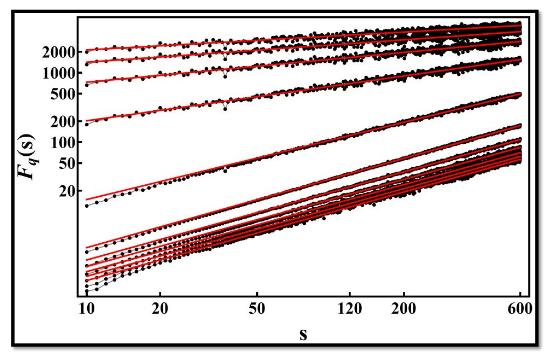
\includegraphics[width=1.0\linewidth]{EDMIIssues/Figures/dfa.png}
	\end{subfigure}
	\caption{Miara fluktuacji w funkcji szerokości segmentu dla różnych wartości parametru $ q $.}
	\label{dfa}
\end{figure} 

\underline{Wielkoskalowa analiza multifraktalna}

\begin{itemize}
	\item Stosujemy przesuwające się i rozszerzające okno
	\item Regresja wykonywana jest tylko wewnątrz aktualnego położenia okna
	\item Ponieważ $ F_q(s) $ jest w skali $ \log-\log $ okno rozszerza się logarytmicznie
	\item Powstaje tzw. powierzchnia Hursta (rys~\ref{wam})
\end{itemize}

\begin{figure} [H]
	\centering
	\begin{subfigure}{.8\textwidth}
		\centering
		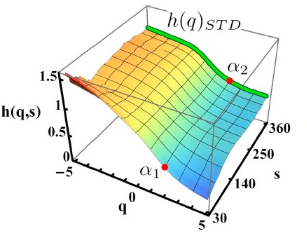
\includegraphics[width=1.0\linewidth]{EDMIIssues/Figures/wam.png}
	\end{subfigure}
	\caption{Miara fluktuacji w funkcji szerokości segmentu oraz wartości parametru $ q $.}
	\label{wam}
\end{figure}